\documentclass[11pt,a4paper]{article}

\usepackage[T1]{fontenc}
\usepackage[utf8]{inputenc}
\usepackage{lmodern}
\usepackage[margin=2.5cm]{geometry}
\usepackage{microtype}
\usepackage{booktabs}
\usepackage{tabularx}
\usepackage{array}
\usepackage{tikz}
\usetikzlibrary{arrows.meta,positioning}
\usepackage{enumitem}
\usepackage[hidelinks]{hyperref}

\setlist{itemsep=2pt,topsep=4pt}
\newcolumntype{L}{>{\raggedright\arraybackslash}X}

\title{Research Method of the Master Thesis\\[4pt]
\large Comparing Autoregressive Models and Recurrent Neural Networks\\
for Short-Term Photovoltaic Power Forecasting}
\author{Eris Allkanjari\\[2pt]
\small Supervisor: Zsolt Saffer}
\date{\today}

\begin{document}
\maketitle

\begin{abstract}
\noindent
Rooftop photovoltaic (PV) systems feed a growing share of electricity into
distribution grids, yet their output fluctuates with cloud cover from one hour
to the next. Grid operators and energy traders therefore depend on reliable
short-term forecasts, and it is still unclear whether recurrent neural networks
justify their higher cost over classical autoregressive models for this task.
This thesis compares autoregressive models (ARIMA, SARIMA, ARIMAX, SARIMAX) with
recurrent networks (LSTM, GRU) for one-step-ahead forecasting of the aggregated
production of 175 rooftop PV systems in Utrecht, the Netherlands, combined with
weather observations from the Royal Netherlands Meteorological Institute (KNMI)
at hourly and 10-minute resolution. The work follows the Cross-Industry Standard
Process for Data Mining (CRISP-DM), complemented by the quality-assurance
practices of CRISP-ML(Q). Its six phases structure the project from problem
definition and data preparation through model tuning and a single held-out test
evaluation to a reproducible, documented forecasting pipeline.
\end{abstract}

\section{Introduction}

A data-driven thesis needs a research method that fixes the order of work,
states what each step must deliver and makes the path from raw data to
conclusions traceable. Process models from data mining provide exactly this.
Section~\ref{sec:literature} summarises the process models described in the
literature, concentrating on their methodological steps, and explains why
CRISP-DM was selected. Section~\ref{sec:application} shows how each CRISP-DM
phase and its tasks are carried out in this thesis.

\section{Research Methods in the Literature}
\label{sec:literature}

\subsection{The KDD process}

The earliest widely cited process model is the Knowledge Discovery in Databases
(KDD) process of Fayyad, Piatetsky-Shapiro and Smyth~\cite{fayyad1996}. They
separate \emph{data mining}, the application of an algorithm to extract
patterns, from the overall \emph{knowledge discovery} process that surrounds it.
The process runs through the steps of selection, preprocessing, transformation,
data mining, and interpretation/evaluation, and it is explicitly iterative: the
results of a later step can send the analyst back to an earlier one. The KDD
process concentrates on the technical treatment of data. It says little about
how a project is anchored in an application problem or how its results are put
into use.

\subsection{CRISP-DM}

The Cross-Industry Standard Process for Data Mining (CRISP-DM) was developed at
the end of the 1990s by a consortium of industrial partners and published as a
step-by-step guide~\cite{chapman2000}. Wirth and Hipp~\cite{wirth2000} and
Shearer~\cite{shearer2000} introduced it to the research and practitioner
communities. CRISP-DM is designed to be independent of the industry sector and
of the tools used. The guide organises the process on four levels of
abstraction: \emph{phases}, \emph{generic tasks}, \emph{specialised tasks} and
\emph{process instances}. The top level consists of six phases, each with a
fixed set of generic tasks and outputs~\cite{chapman2000}:

\begin{enumerate}[label=\arabic*.]
  \item \textbf{Business understanding:} determine the business objectives,
        assess the situation (resources, constraints, risks), translate the
        objectives into data mining goals with success criteria, and produce a
        project plan.
  \item \textbf{Data understanding:} collect the initial data, describe it,
        explore it, and verify its quality.
  \item \textbf{Data preparation:} select, clean, construct, integrate and
        format the data into the final modelling dataset.
  \item \textbf{Modelling:} select modelling techniques, generate a test design,
        build the models, and assess them against the technical criteria.
  \item \textbf{Evaluation:} evaluate the results against the business
        objectives, review the process, and determine the next steps.
  \item \textbf{Deployment:} plan deployment, plan monitoring and maintenance,
        produce the final report, and review the project.
\end{enumerate}

\noindent
The sequence of phases is not rigid (Figure~\ref{fig:crispdm}). Moving back and
forth between business and data understanding, and between data preparation and
modelling, is the normal case, and the outer cycle expresses that a finished
project usually raises new questions~\cite{chapman2000,wirth2000}. The guide
also allows deployment to be as simple as producing a report, which matters for
academic projects that do not end in an operational system.

\begin{figure}[ht]
\centering
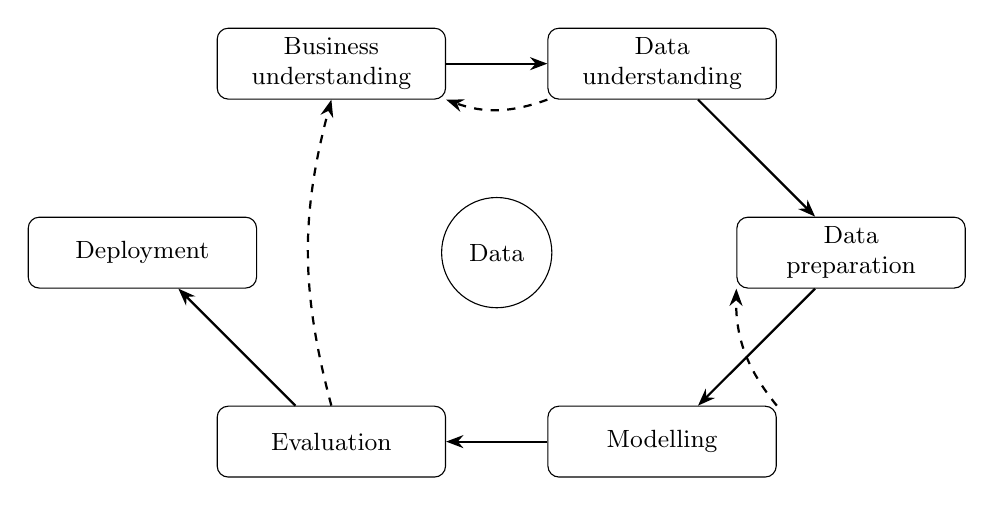
\begin{tikzpicture}[
  phase/.style={draw, rounded corners, align=center, minimum width=2.9cm,
                minimum height=0.9cm, font=\small},
  arr/.style={-{Stealth[length=2.2mm]}, thick},
  back/.style={-{Stealth[length=2.2mm]}, thick, dashed}]
  \node[phase] (bu) at (0,2.4)    {Business\\understanding};
  \node[phase] (du) at (4.2,2.4)  {Data\\understanding};
  \node[phase] (dp) at (6.6,0)    {Data\\preparation};
  \node[phase] (mo) at (4.2,-2.4) {Modelling};
  \node[phase] (ev) at (0,-2.4)   {Evaluation};
  \node[phase] (de) at (-2.4,0)   {Deployment};
  \node[draw, circle, minimum size=1.4cm, font=\small] (data) at (2.1,0) {Data};
  \draw[arr] (bu) -- (du);
  \draw[arr] (du) -- (dp);
  \draw[arr] (dp) -- (mo);
  \draw[arr] (mo) -- (ev);
  \draw[arr] (ev) -- (de);
  \draw[back] (du.south west) to[bend left=20] (bu.south east);
  \draw[back] (mo.north east) to[bend left=20] (dp.south west);
  \draw[back] (ev.north) to[bend left=15] (bu.south);
\end{tikzpicture}
\caption{The six CRISP-DM phases after~\cite{chapman2000}. Solid arrows show
the main sequence, dashed arrows the most frequent iterations.}
\label{fig:crispdm}
\end{figure}

\subsection{Comparisons of process models}

Azevedo and Santos~\cite{azevedo2008} compare CRISP-DM with the KDD process and
with SEMMA (Sample, Explore, Modify, Model, Assess), the model proposed by SAS.
They find that the three are largely equivalent in their technical core: SEMMA
and CRISP-DM can both be mapped onto the KDD steps. The difference is that
CRISP-DM adds a business understanding phase before the data work and a
deployment phase after it. The broader surveys by Kurgan and
Musilek~\cite{kurgan2006} and by Mariscal, Marb\'an and
Fern\'andez~\cite{mariscal2010} reach a similar conclusion across a wider set of
process models. The models differ mainly in how finely they divide the work and
in whether they cover the project context, while the core sequence from data
understanding to evaluation is shared. Both surveys identify CRISP-DM as the
most widely adopted model in practice.

\subsection{Use and adaptation in practice}

Plotnikova, Dumas and Milani~\cite{plotnikova2020} review over two hundred
publications and find that data mining methodologies are mostly applied as they
are, but that projects regularly adapt them, for example by extending a phase or
by integrating domain-specific steps. Schr\"oer, Kruse and
G\'omez~\cite{schroer2021} review applications of CRISP-DM specifically. They
show that published projects describe the early, data-related phases in detail,
while the deployment phase is often treated only briefly. Shimaoka, Ferreira and
Goldman~\cite{shimaoka2024} trace how later data science process frameworks
build on CRISP-DM, which remains the common reference point.

\subsection{Extensions for machine learning and engineering data}

Two extensions address gaps relevant to this thesis. Studer et
al.~\cite{studer2021} propose CRISP-ML(Q), which adapts CRISP-DM to machine
learning projects. It merges business and data understanding into one phase,
names the phases data preparation, model engineering, model evaluation and model
deployment, and adds monitoring and maintenance. Its main contribution is a
quality-assurance methodology: for every task, requirements and constraints are
defined, risks that could compromise the result are identified, and specific
quality-assurance methods are chosen to mitigate them. Wiemer, Drowatzky and
Ihlenfeldt~\cite{wiemer2019} extend CRISP-DM for engineering applications with
DMME, adding explicit steps for technical understanding and for planning the
acquisition of data from physical systems, which CRISP-DM assumes to be already
available.

\subsection{Limitations and choice of method}

Mart\'inez-Plumed et al.~\cite{martinezplumed2021} ask whether CRISP-DM still
fits modern data science. They conclude that the process model remains
appropriate for goal-directed projects with a clear question, while exploratory
projects follow more varied trajectories that a fixed sequence of phases
describes poorly.

This thesis is a goal-directed project: the research question, the data sources
and the model families are fixed in advance. CRISP-DM is therefore selected as
the research method for three reasons. First, its business understanding phase
forces the research question and the success criteria to be fixed before any
model is fitted. Second, its separation of modelling and evaluation matches the
experimental requirement that models are tuned on validation data and judged on
untouched test data. Third, it is the most widely used and documented process
model~\cite{kurgan2006,mariscal2010,schroer2021}, which makes the work easy to
follow and to reproduce. Because the project builds its own dataset from
physical measurements and trains machine learning models, two elements from the
extensions are adopted: the task-level quality assurance of
CRISP-ML(Q)~\cite{studer2021} and the attention to data acquisition of
DMME~\cite{wiemer2019}.

\section{Application of CRISP-DM in the Thesis}
\label{sec:application}

This section follows the six phases and their generic tasks. Table~\ref{tab:mapping}
summarises the mapping, and the subsections describe each phase.

\begin{table}[ht]
\centering
\small
\begin{tabularx}{\textwidth}{@{}p{2.6cm}LL@{}}
\toprule
\textbf{Phase} & \textbf{Generic tasks~\cite{chapman2000}} & \textbf{Activities in this thesis} \\
\midrule
Business understanding & Objectives, situation, data mining goals, plan
  & Research questions; one-step-ahead horizon; error metrics and baselines as
    success criteria; plan of experiments \\
Data understanding & Collect, describe, explore, verify quality
  & PV data of 175 systems and KNMI weather; autocorrelation, stationarity and
    cross-correlation analyses; coverage and outage audit \\
Data preparation & Select, clean, construct, integrate, format
  & Interval aggregation; causal gap filling; time encoding; timestamp
    alignment of PV and weather; chronological split and scaling \\
Modelling & Technique, test design, build, assess
  & ARIMA family and LSTM/GRU; rolling-origin validation; hyperparameter grids;
    robust selection rule \\
Evaluation & Evaluate results, review process, next steps
  & Single test-set comparison; feature significance; documented iterations
    back to earlier phases \\
Deployment & Plan deployment and monitoring, final report, review
  & Reproducible command-line pipeline; protocol version tags; thesis report;
    outlook on operational use \\
\bottomrule
\end{tabularx}
\caption{Mapping of the CRISP-DM phases onto the work in this thesis.}
\label{tab:mapping}
\end{table}

\subsection{Business understanding}

The objective is to support grid operation and energy trading with short-term
forecasts of rooftop PV output. It is translated into three research questions:
(i) whether recurrent networks forecast aggregated PV production more accurately
than autoregressive models one step ahead, (ii) whether weather inputs improve
each model family, and (iii) how the comparison changes between hourly and
10-minute resolution. The data mining goal is a fair, reproducible comparison
under identical conditions. Success criteria are defined before modelling: the
mean absolute error (MAE) as the primary metric, the root mean square error
(RMSE), the MAE normalised by a reference capacity (NMAE) to allow comparison
with other sites, and the mean absolute percentage error (MAPE) restricted to
daylight periods where it is meaningful. Every model must also be measured
against persistence and a seasonal-naive baseline, following the
recommendations for solar forecast verification of Yang et al.~\cite{yang2020}.
The situation assessment identifies the main constraints: a PV fleet whose size
changes over the record, and the high computational cost of seasonal
autoregressive models at 10-minute resolution.

\subsection{Data understanding}

\emph{Collect.} The target is the aggregated production of 175 residential
rooftop systems in Utrecht, measured at one-minute resolution from 2014 to
2017~\cite{visser2022}. Weather data come from the KNMI station De Bilt, both as
the validated hourly product and as 10-minute in-situ observations.
\emph{Describe.} Variables, units and resolutions are documented, including the
convention each source uses to label time intervals. \emph{Explore.}
Autocorrelation and partial autocorrelation functions and stationarity tests
inform the autoregressive orders and the seasonal period. The cross-correlation
between PV production and radiation is used to check that both sources describe
the same interval. \emph{Verify quality.} The share of systems reporting in each
interval is recorded as an observation-coverage measure, which reveals
acquisition outages and the shrinking fleet. Gaps in the weather record are
counted and located. Following DMME~\cite{wiemer2019}, the acquisition of the
data is documented as carefully as the data itself, since the dataset is
assembled within the thesis.

\subsection{Data preparation}

\emph{Select.} The target and five weather variables (radiation, cloud cover,
temperature, wind speed, humidity) are selected. \emph{Clean.} Negative
production is clipped at zero. Missing values are filled only forward in time,
so that imputation can never carry future information into an earlier
period. \emph{Construct.} One-minute power readings are converted to interval
energy. The hourly dataset is aggregated from the 10-minute data following KNMI's
own hourly definitions, and the time of day is encoded as a sine and cosine pair
so that midnight is not an artificial discontinuity. \emph{Integrate.} PV and
weather are merged after both are relabelled to interval start, and the build
stops automatically if the cross-correlation does not peak at lag zero.
\emph{Format.} The data are split chronologically into 65\% training, 15\%
validation and 20\% test, and scalers are fitted on the training split only.
In terms of CRISP-ML(Q)~\cite{studer2021}, the main risk addressed in this phase
is information leakage, and causal imputation, train-only scaling and the
alignment check are the corresponding quality-assurance measures.

\subsection{Modelling}

\emph{Select techniques.} Two families are modelled: autoregressive models in
the Box--Jenkins tradition~\cite{box2015} (ARIMA, SARIMA, and the variants with
exogenous weather inputs, ARIMAX and SARIMAX), and recurrent networks, namely
LSTM~\cite{hochreiter1997} and GRU~\cite{cho2014}. \emph{Generate test design.}
Forecasts are produced one step ahead with a rolling origin, as recommended for
out-of-sample evaluation by Tashman~\cite{tashman2000}. Model selection uses the
validation split only, and the test split is used once at the very end.
Validation errors are computed per calendar month and averaged, so that the
high-production summer months do not dominate. \emph{Build.} Grids of model
orders, history window lengths and network hyperparameters are evaluated.
Recurrent networks are trained with early stopping under three fixed random
seeds and reported as the mean across seeds, so that a favourable
initialisation cannot flatter a result. \emph{Assess.} Autoregressive fits that
do not converge are rejected. Instead of taking the raw minimum, a selection
rule accepts every candidate within 2\% of the best validation MAE and prefers
the more stable one among them, which reduces sensitivity to noise. This
addresses a concern raised by Makridakis et al.~\cite{makridakis2018}, that
comparisons between statistical and machine learning methods are only credible
under identical and transparent evaluation conditions.

\subsection{Evaluation}

\emph{Evaluate results.} The selected models are retrained on training and
validation data and evaluated once on the test period, against the success
criteria defined in the business understanding phase. Errors are additionally
reported separately for day and night hours, because night hours are trivial to
forecast and would otherwise dilute the error. A sensitivity analysis repeats
the comparison on intervals with adequate observation coverage. The
contribution of each input group is measured by removing it and testing the
change in error with a block bootstrap and a correction for multiple testing.

\emph{Review process.} This task is where the iterative nature of CRISP-DM
becomes concrete. Two examples from the project illustrate it. First, the
cross-correlation analysis showed that the weather data were labelled one
interval later than the PV data, so the work returned to data preparation to
realign the sources, and all experiments were repeated. Second, the review of
seed-level test results showed that the final retraining of one network type
was unstable, so the work returned to modelling to adjust the training
procedure. To make such loops safe, each stage writes a protocol version into
its results, and later stages refuse results produced under an outdated
protocol. \emph{Determine next steps.} Each review ends with a documented
decision to proceed or to repeat earlier phases.

\subsection{Deployment}

The thesis does not end in an operational forecasting service. Following the
guide's allowance for report-based deployment~\cite{chapman2000}, the
deployment phase delivers a reproducible pipeline that rebuilds the datasets and
reruns every experiment from the command line, its documentation, and the final
thesis report. The monitoring and maintenance task is addressed as an outlook:
the thesis discusses how often models would need retraining and how the
changing fleet size would affect an operational system. This also responds to
the observation of Schr\"oer et al.~\cite{schroer2021} that deployment is often
neglected in CRISP-DM applications. The final project review compares the
results with the research questions and records the lessons learned.

\section{Summary}

CRISP-DM provides the research method of this thesis. Its six phases fix the
research question and success criteria before modelling, separate model
selection from final evaluation, and make the necessary iterations explicit and
traceable. Elements of CRISP-ML(Q) and DMME complement it with task-level
quality assurance and with documentation of the data acquisition, which are
essential when a dataset is assembled from physical measurements and machine
learning models are compared with classical statistical ones.

\begin{thebibliography}{99}
\small

\bibitem{azevedo2008}
A.~Azevedo and M.~F. Santos,
``KDD, SEMMA and CRISP-DM: a parallel overview,''
in \emph{Proc. IADIS European Conference on Data Mining}, 2008, pp.~182--185.

\bibitem{box2015}
G.~E.~P. Box, G.~M. Jenkins, G.~C. Reinsel, and G.~M. Ljung,
\emph{Time Series Analysis: Forecasting and Control}, 5th~ed.
Hoboken, NJ: Wiley, 2015.

\bibitem{chapman2000}
P.~Chapman, J.~Clinton, R.~Kerber, T.~Khabaza, T.~Reinartz, C.~Shearer, and
R.~Wirth,
\emph{CRISP-DM 1.0: Step-by-Step Data Mining Guide}.
CRISP-DM Consortium, 2000.

\bibitem{cho2014}
K.~Cho, B.~van Merri\"enboer, C.~Gulcehre, D.~Bahdanau, F.~Bougares,
H.~Schwenk, and Y.~Bengio,
``Learning phrase representations using RNN encoder--decoder for statistical
machine translation,''
in \emph{Proc. EMNLP}, 2014, pp.~1724--1734.

\bibitem{fayyad1996}
U.~Fayyad, G.~Piatetsky-Shapiro, and P.~Smyth,
``From data mining to knowledge discovery in databases,''
\emph{AI Magazine}, vol.~17, no.~3, pp.~37--54, 1996.

\bibitem{hochreiter1997}
S.~Hochreiter and J.~Schmidhuber,
``Long short-term memory,''
\emph{Neural Computation}, vol.~9, no.~8, pp.~1735--1780, 1997.

\bibitem{kurgan2006}
L.~A. Kurgan and P.~Musilek,
``A survey of knowledge discovery and data mining process models,''
\emph{The Knowledge Engineering Review}, vol.~21, no.~1, pp.~1--24, 2006.

\bibitem{makridakis2018}
S.~Makridakis, E.~Spiliotis, and V.~Assimakopoulos,
``Statistical and machine learning forecasting methods: Concerns and ways
forward,''
\emph{PLOS ONE}, vol.~13, no.~3, e0194889, 2018.

\bibitem{mariscal2010}
G.~Mariscal, \'O.~Marb\'an, and C.~Fern\'andez,
``A survey of data mining and knowledge discovery process models and
methodologies,''
\emph{The Knowledge Engineering Review}, vol.~25, no.~2, pp.~137--166, 2010.

\bibitem{martinezplumed2021}
F.~Mart\'inez-Plumed, L.~Contreras-Ochando, C.~Ferri, J.~Hern\'andez-Orallo,
M.~Kull, N.~Lachiche, M.~J. Ram\'irez-Quintana, and P.~Flach,
``CRISP-DM twenty years later: From data mining processes to data science
trajectories,''
\emph{IEEE Transactions on Knowledge and Data Engineering}, vol.~33, no.~8,
pp.~3048--3061, 2021.

\bibitem{plotnikova2020}
V.~Plotnikova, M.~Dumas, and F.~Milani,
``Adaptations of data mining methodologies: a systematic literature review,''
\emph{PeerJ Computer Science}, vol.~6, e267, 2020.

\bibitem{schroer2021}
C.~Schr\"oer, F.~Kruse, and J.~M. G\'omez,
``A systematic literature review on applying CRISP-DM process model,''
\emph{Procedia Computer Science}, vol.~181, pp.~526--534, 2021.

\bibitem{shearer2000}
C.~Shearer,
``The CRISP-DM model: The new blueprint for data mining,''
\emph{Journal of Data Warehousing}, vol.~5, no.~4, pp.~13--22, 2000.

\bibitem{shimaoka2024}
A.~M. Shimaoka, R.~C. Ferreira, and A.~Goldman,
``The evolution of CRISP-DM for data science: Methods, processes and
frameworks,''
\emph{SBC Reviews on Computer Science}, 2024.

\bibitem{studer2021}
S.~Studer, T.~B. Bui, C.~Drescher, A.~Hanuschkin, L.~Winkler, S.~Peters, and
K.-R. M\"uller,
``Towards CRISP-ML(Q): A machine learning process model with quality assurance
methodology,''
\emph{Machine Learning and Knowledge Extraction}, vol.~3, no.~2, pp.~392--413,
2021.

\bibitem{tashman2000}
L.~J. Tashman,
``Out-of-sample tests of forecasting accuracy: an analysis and review,''
\emph{International Journal of Forecasting}, vol.~16, no.~4, pp.~437--450,
2000.

\bibitem{visser2022}
L.~Visser, B.~Elsinga, T.~AlSkaif, and W.~van Sark,
``Open-source quality control routine and multi-year power generation data of
175 PV systems,''
\emph{Journal of Renewable and Sustainable Energy}, vol.~14, 2022,
doi:~10.1063/5.0100939.

\bibitem{wiemer2019}
H.~Wiemer, L.~Drowatzky, and S.~Ihlenfeldt,
``Data mining methodology for engineering applications (DMME)---A holistic
extension to the CRISP-DM model,''
\emph{Applied Sciences}, vol.~9, no.~12, 2407, 2019.

\bibitem{wirth2000}
R.~Wirth and J.~Hipp,
``CRISP-DM: Towards a standard process model for data mining,''
in \emph{Proc. 4th International Conference on the Practical Applications of
Knowledge Discovery and Data Mining}, 2000, pp.~29--39.

\bibitem{yang2020}
D.~Yang, S.~Alessandrini, J.~Antonanzas, F.~Antonanzas-Torres, V.~Badescu,
H.~G. Beyer, R.~Blaga, J.~Boland, J.~M. Bright, C.~F.~M. Coimbra, et~al.,
``Verification of deterministic solar forecasts,''
\emph{Solar Energy}, vol.~210, pp.~20--37, 2020.

\end{thebibliography}

\end{document}
